\documentclass[11pt]{beamer}
\usetheme{CambridgeUS}
\usepackage[utf8]{inputenc}
\usepackage{amsmath}
\usepackage{amsfonts}
\usepackage{amssymb}
\usepackage[
backend=biber,
style=alphabetic,
citestyle=authoryear
]{biblatex}
\usepackage{array}
\usepackage{xcolor}

% Footnote without number
\newcommand\blfootnote[1]{%
  \begingroup
  \renewcommand\thefootnote{}\footnote{#1}%
  \addtocounter{footnote}{-1}%
  \endgroup
}
\def\boxit#1{%
  \smash{\color{red}\fboxrule=1pt\relax\fboxsep=2pt\relax%
  \llap{\rlap{\fbox{\vphantom{0}\makebox[#1]{}}}~}}\ignorespaces
}
\addbibresource{stats.bib}
\title[Bioestatística II] %optional
{Teste t de amostra única}

\subtitle{CGF2046 - Bioestatística II}

\author[da Silva, Ricardo] % (optional, for multiple authors)
{R. ~R. ~da Silva\inst{1}}

\institute[FCFRP] % (optional)
{
  \inst{1}%
  Departamento de Ciências BioMoleculares\\
  Faculdade de Ciências Farmacêuticas

}

\date{\today} % (optional)

\titlegraphic{
\includegraphics[width=5.8cm]{figs/logo_final}} 

\begin{document}

%\begin{frame}
%\titlepage
%\end{frame}

%\begin{frame}
%\tableofcontents
%\end{frame}

\begin{frame}
\titlepage
\end{frame}

\begin{frame}
\label{contents}
\frametitle{Sumário}
\tableofcontents
\end{frame}

\setbeamercovered{transparent}
\begin{frame}
\frametitle{Objetivos de Aprendizado\footcite{carlson2017introduction}}
  Depois de assitir essa aula e fazer as atividades complementares, você será capaz de:
  \\~\\
  \begin{itemize}
  \uncover<1->{\item
    Explicar quando um t de amostra única deve ser usado em vez de z para uma média amostral;}
  \uncover<2->{\item
    Escrever hipóteses nulas unicaudais e bicaudais e hipóteses de pesquisa usando parâmetros populacionais e também textualmente;}
   \uncover<3->{\item
    Calcular os graus de liberdade e definir a região crítica para testes t unicaudais e bicaudais de amostra única;}
   \uncover<4->{\item
    Explicar por que um z para um teste de média amostral e um teste t de amostra única têm regiões críticas diferentes;}
   \uncover<5->{\item
    Calcular um t de amostra única manualmente e usando \textit{software};}
   \uncover<6->{\item
    Determinar se você deve ou não rejeitar a hipótese nula;}
   \uncover<7->{\item
    Calcular e interpretar um tamanho de efeito (d);}
   \uncover<8->{\item
    Interpretar a saída do \textit{software} para um t de amostra única.}            
  \end{itemize}
\end{frame}

\section{Introdução ao teste t}
\setbeamercovered{transparent}
\begin{frame}
\frametitle{Contexto}
No último capítulo, você aprendeu a usar a variável padrão z como estatística da média amostral para testar uma hipótese nula. \textit{calcular o z para uma média amostral, você deve conhecer o desvio padrão da população ($\sigma$)}. \\~\\ 
  
\textit{Porém, na maioria das situações de pesquisa, o desvio padrão da população não é conhecido}. Neste capítulo, você aprenderá como usar a estatística t de amostra única quando não souber o desvio padrão da população.
\end{frame}

\setbeamercovered{transparent}
\begin{frame}
\frametitle{Contexto}
O teste t de amostra única é logicamente idêntico ao z para uma média amostral.

\begin{center}
\small
\begin{tabular}{ccc} 
 \hline
 &	z para uma média amostral & teste t de amostra única\\
 \hline
Fórmula & $z = \frac{\bar{x}-\mu}{SEM_p}$ & $t =\frac{\bar{x}-\mu}{SEM_a}$\\
 &  & \\
Cálculo do erro amostral & $SEM_p = \frac{\sigma}{\sqrt{N}}$ & $SEM_a = \frac{DP}{\sqrt{N}}$\\
(erro padrão da média) &  & \\
 \hline
\end{tabular}
\end{center}

\end{frame}

\setbeamercovered{transparent}
\begin{frame}
\frametitle{Contexto}
O valor crítico para um teste z unilateral com $\alpha = 0.05$ é sempre +1.65 ou -1.65. 
\\~\\
\textit{Por outro lado, os valores críticos para um teste t unilateral com $\alpha = 0.05$ mudarão com base em quantos elementos estão na amostra}. A consequência importante das curvas t terem um formato diferente para cada tamanho de amostra é que os valores críticos que definem a região crítica são diferentes para cada tamanho de amostra (isto é, N). 
\\~\\
À medida que N aumenta, o valor crítico de t fica mais próximo do valor crítico de z.
\end{frame}

\setbeamercovered{transparent}
\begin{frame}
\frametitle{Comparação de curvas t}

\begin{center}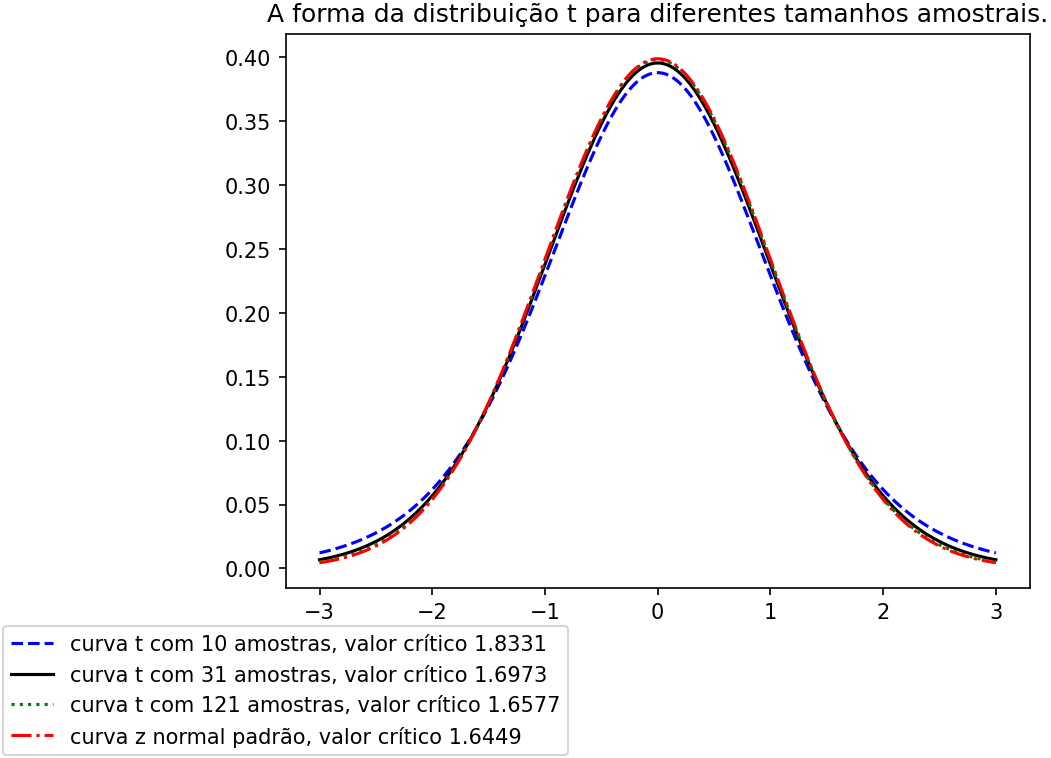
\includegraphics[width=0.8\linewidth]{figs/comp_curvas_t.png} \end{center}

\end{frame}


\setbeamercovered{transparent}
\begin{frame}
\frametitle{Teste t unicaudal de amostra única}

\textbf{Exemplo:} O salário inicial médio estimado dos alunos é significativamente superior ao salário inicial real dos cursos de farmácia?

\begin{itemize}
\item Sabe se que a distribuição dos salários iniciais dos formandos em farmácia é normalmente distribuída com uma média $\mu = 3000$ por mês;
\item
   Salários iniciais mensais esperados de 15 alunos: 3500, 4200, 2500, 3200, 2700, 2000, 2500, 4100, 5000, 4200, 2900, 3900, 4000, 5000 e 5500;
\item
  Média amostral de $\bar{x} = 3680$.
\end{itemize}

Optamos por um teste unilateral. Também escolhemos um \(\alpha=0.05\).

\end{frame}

\setbeamercovered{transparent}
\begin{frame}
\frametitle{Etapa 1: examinar as pressuposições estatísticas}

Todos os testes de hipóteses são baseados em suposições específicas e, se essas suposições forem violadas, esses testes podem produzir resultados enganosos.\\~\\
Os quatro pressupostos básicos são:

\begin{enumerate}
\item independência dos dados;
\item medição apropriada das variáveis para análise;
\item normalidade das distribuições;
\item homogeneidade da variância.
\end{enumerate}

\end{frame}

\setbeamercovered{transparent}
\begin{frame}
\frametitle{Etapa 1: examinar as pressuposições estatísticas}

Os quatro pressupostos básicos são:

\begin{enumerate}
\item \textbf{independência dos dados:} as expectativas de salários um estudante é independente das expectativas de todos os outros;
\item \textbf{medição apropriada:} variável independente (VI) \(\Rightarrow\) expectativas dos estudantes versus salários reais, variável dependente (VD) \(\Rightarrow\) o salário mensal esperado, é medido em como uma variável quantitativa;
\item \textbf{normalidade das distribuições:} população de salários esperados dos formandos em farmácia é normalmente distribuida;
\item \textbf{homogeneidade da variância:} é seguro assumir que o desvio padrão da amostra será semelhante ao desvio padrão da população?
\end{enumerate}

\end{frame}

\setbeamercovered{transparent}
\begin{frame}
\frametitle{Etapa 2: expor as hipóteses nulas e de pesquisa simbolicamente e verbalmente}

Um valor t em uma região crítica positiva indicaria que a média da amostra é significativamente maior do que o valor real de 3000/mês.

\begin{center}
\begin{tabular}{ m{2cm}|m{2cm}|m{3cm}|m{3cm} } 
 \hline
 Tipo de Hipótese & Simbólico & Vebal & Diferença entre médias amostral e populacional\\
  \hline
 Hipótese nula & $\mu_{farma}=3000;$ & Salário estimado $\approx$ 3000 & Erro amostral \\ 
 Hipótese de pesquisa & $\mu_{farma}>3000.$ & Salário estimado $>$ 3000 & Estudantes superestimam salário  \\ 
 \hline
 \hline
\end{tabular}
\end{center}

\end{frame}

\begin{frame}
\frametitle{Etapa 3: Use o tamanho da amostra para calcular os graus de liberdade e defina as regiões críticas}
Depois de saber o tamanho da amostra de um estudo, você precisa calcular seus graus de liberdade (gl). Para o teste t de amostra única, a fórmula para o gl é \textit{gl = N - 1}. Portanto, neste caso,
\[gl = 15 - 1 = 14\]

\begin{columns}
\begin{column}{0.5\textwidth}
   Excerto da tabela t\\~\\

\begin{center}
\begin{tabular}{ccc} 
 \hline
gl & $\alpha = .05$ & $\alpha = .01$\\
13 & 1.770900 & 2.650300\\
\boxit{1.7in} 14 & 1.761300 & 2.624500\\
15 & 1.753100 & 2.602500\\
 \hline
\end{tabular}
\end{center}   
   
   
\end{column}
\begin{column}{0.5\textwidth}  %%<--- here
   \begin{itemize}
   \item O valor de corte de \(\alpha= .05\) define a região crítica, os valores t são improváveis se o valor nulo for verdadeiro.
   \end{itemize}
\end{column}
\end{columns}
\end{frame}

\setbeamercovered{transparent}
\begin{frame}
\frametitle{Etapa 4: calcular a estatística do teste (teste t de amostra única)}
\begin{itemize}
\item 4a. Calcule o desvio observado entre a média amostral e a média da população
\[\bar{x} - \mu = 3680-3000 = 680\]
\item 4b. Calcule o desvio esperado devido ao erro de amostragem
\[Var(X) = \frac{1}{N-1}\sum_{i=1}^n(X_i - \bar{X})^2 = 1078857.143\]
\[SEM_a = \frac{DP}{\sqrt{N}} = \frac{1038.680}{\sqrt{15}} = 268.186\]
\item 4c. Calcule o z para uma média amostral
\[t = \frac{(\bar{x} - \mu)}{SEM_a} = \frac{(3680-3000)}{268.186} = 2.54.\]
\end{itemize}
\end{frame}

\setbeamercovered{transparent}
\begin{frame}
\frametitle{Etapa 4: calcular a estatística do teste (teste t de amostra única)}
O valor t obtido de 2.54 é mais extremo que o valor crítico de 1.7613, portanto esse valor de t está localizado na região de rejeição (ou seja, a região crítica).
\begin{center}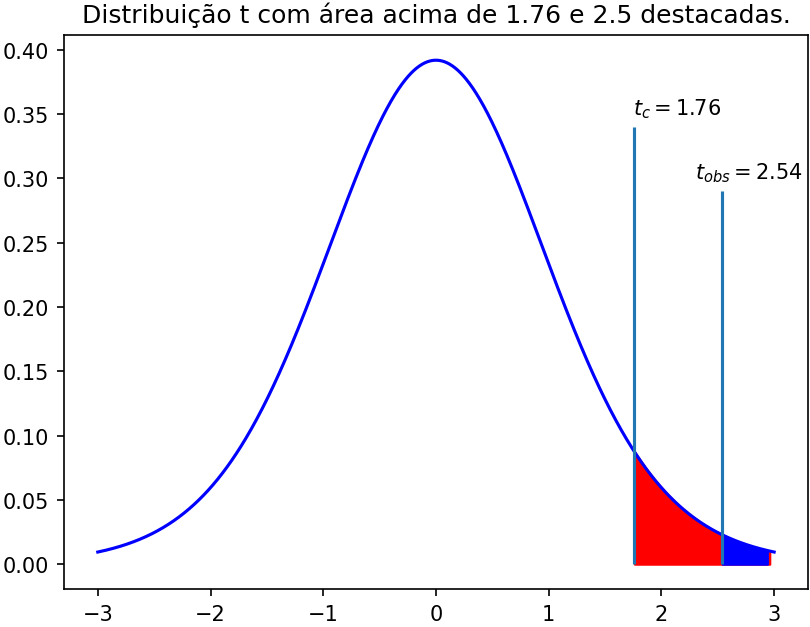
\includegraphics[width=0.55\linewidth]{figs/regiao_critica_observada_t} \end{center}

\end{frame}


\setbeamercovered{transparent}
\begin{frame}
\frametitle{Etapa 5: calcule o tamanho do efeito e descreva se o seu grau}
Um tamanho de efeito é um índice da diferença entre a média da amostra e a média da população. A estatística de tamanho do efeito normalmente usada ao comparar duas médias é d. 
\begin{align*}
d &= \frac{Desvio\quad observado\quad entre\quad as\quad medias}{Desvio\quad padrao}\\
  &= \frac{\bar{x}-\mu}{DP} = \frac{3680 - 3000}{1038.68} = 0.65
\end{align*}

\end{frame}

\setbeamercovered{transparent}
\begin{frame}
\frametitle{Etapa 5: calcule o tamanho do efeito e descreva se o seu grau}
A melhor maneira de interpretar qualquer tamanho de efeito é compará-lo com os tamanhos de efeito produzidos por estudos semelhantes na literatura de pesquisa. Se você não conseguir encontrar estudos semelhantes na literatura para fornecer uma referência, poderá usar as diretrizes gerais sugeridas por Cohen (1992) para interpretar os tamanhos dos efeitos na Tabela 6.2.

\begin{center}
\begin{tabular}{cc} 
 \hline
d  & Tamanho estimado do efeito\\
 \hline
Perto de 0.2 & Pequeno \\
Perto de 0.5 & Médio \\
Perto de 0.8 & Grande \\
 \hline
\end{tabular}
\end{center}   

\end{frame}

\setbeamercovered{transparent}
\begin{frame}
\frametitle{Etapa 6: Interpretando os Resultados do Teste de Hipóteses}

Declaração resumida sobre o teste estatístico acima:\\~\\

O salário médio mensal esperado para formandos em farmácia ($\bar{x} = 680, DP = 1038.68$) foi significativamente maior do que o salário inicial real de 3.000 Reais, t(14) = 2.54, \(p < 0.05\), d = 0.65. Esta análise sugere que os formandos em farmácia tendem a superestimar bastante os salários iniciais que podem esperar após a formatura.\\~\\

Geralmente, você deve fornecer o valor exato de p, se souber. Em alguns casos, você não saberá disso e então escreveria "\(p < 0.05\)" se rejeitou a hipótese nula ou "\(p > 0.05\)" se não rejeitou a hipótese nula.
\end{frame}

\begin{frame}
\frametitle{Exemplo de teste t de amostra única de duas caudas (bicaudal)}
\textbf{Exemplo:} Os alunos são igualmente otimistas ao estimar os salários iniciais dos outros? 
Você não tem certeza se os alunos superestimarão ou subestimarão os salários iniciais dos outros e, portanto, você deve fazer um teste bicaudal em vez de um teste unilateral.\\~\\ 

A hipótese de pesquisa bicaudal afirma que o salário médio mensal estimado será superior a 3000 Reais ou inferior a 3000 Reais. \\~\\

Assim, as hipóteses de pesquisa bicaudais possuem duas regiões críticas, uma na cauda positiva e outra na cauda negativa. \\~\\

A escolha entre um teste unicaudal ou bicaudal pode ter um impacto dramático na(s) região(ões) crítica(s) e, portanto, sua decisão sobre usar um teste unicaudal ou bicaudal pode influenciar se você rejeita ou não a hipótese nula do teste. \\~\\

Portanto, se a sua hipótese de pesquisa for direcional, é vantajoso usar um teste unilateral em vez de um teste bicaudal.
\end{frame}

\begin{frame}
\frametitle{Exemplo de teste t de amostra únical de duas caudas (bicaudal)}
Com amostra  N=15 um teste unilateral com $\alpha = 0.05$, tem valor crítico seria +1.7613 \(\Rightarrow\) se o valor t obtido fosse +1.8 a hipótese seria rejeitada. \\~\\
Em um teste bicaudal, seus valores t críticos seriam +2.1448 e -2.1448, a hipótese nula não seria rejeitada.
\begin{columns}
\begin{column}{0.5\textwidth}
   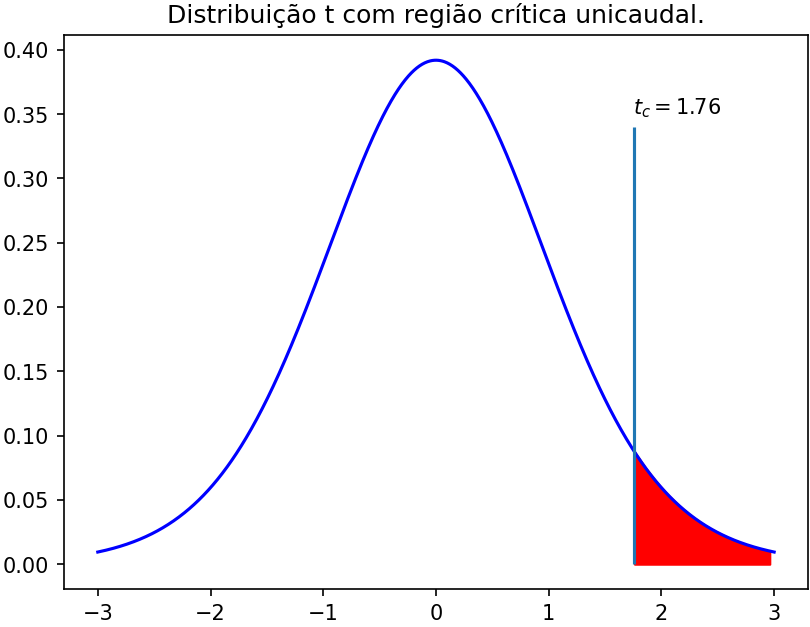
\includegraphics[width=1\linewidth]{figs/regiao_critica_unicaudal_t}
\end{column}
\begin{column}{0.5\textwidth}  %%<--- here
   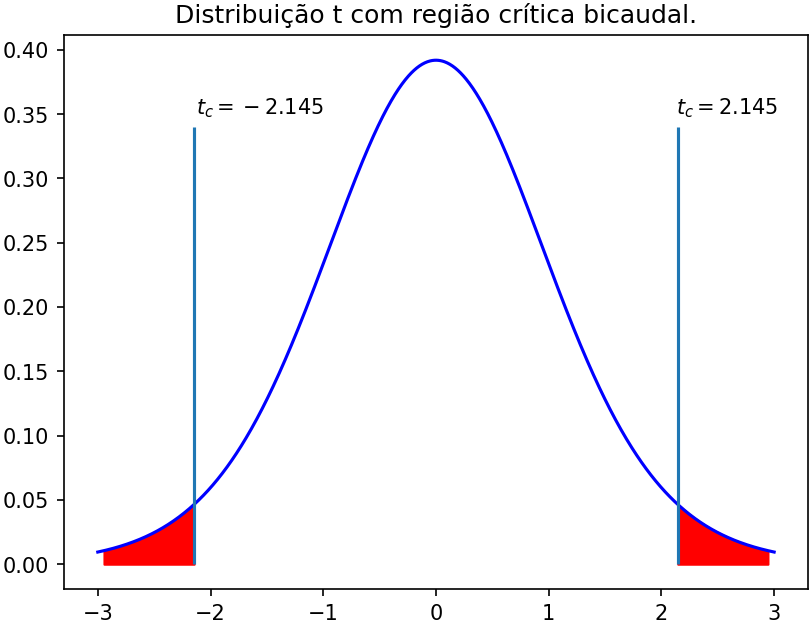
\includegraphics[width=1\linewidth]{figs/regiao_critica_bicaudal_t}
\end{column}
\end{columns}
\end{frame}

\setbeamercovered{transparent}
\begin{frame}
\frametitle{Teste t bicaudal de amostra única}

\textbf{Exemplo:} Você recruta 15 estudantes de farmácia diferentes e pede-lhes que estimem o salário médio mensal que um estudante de farmácia típico pode esperar em seu primeiro emprego após a formatura.
\begin{itemize}
\item Sabe se que a distribuição dos salários iniciais dos formandos em farmácia é normalmente distribuída com uma média $\mu = 3000$ por mês;
\item
   Salários iniciais mensais esperados de 15 alunos: 3400, 3500, 2500, 3200, 2700, 2000, 2500, 3300, 3200, 3000, 2900, 3900, 3800, 3900 e 3600;
\item
  Média amostral de $\bar{x} = 3680$.
\end{itemize}

Optamos por um teste bilateral. Também escolhemos um \(\alpha=0.05\).

\end{frame}



\setbeamercovered{transparent}
\begin{frame}
\frametitle{Etapa 1: examinar as pressuposições estatísticas}

O novo estudo parece atender a todas as quatro suposições estatísticas.

\begin{enumerate}
\item \textbf{independência dos dados:} as expectativas de salários um estudante é independente das expectativas de todos os outros;
\item \textbf{medição apropriada:} variável independente (VI) \(\Rightarrow\) expectativas dos estudantes versus salários reais, variável dependente (VD) \(\Rightarrow\) o salário mensal esperado, é medido em como uma variável quantitativa;
\item \textbf{normalidade das distribuições:} população de salários esperados dos formandos em farmácia é normalmente distribuida;
\item \textbf{homogeneidade da variância:} é seguro assumir que o desvio padrão da amostra será semelhante ao desvio padrão da população?
\end{enumerate}

\end{frame}

\setbeamercovered{transparent}
\begin{frame}
\frametitle{Etapa 2: expor as hipóteses nulas e de pesquisa simbolicamente e verbalmente}

Um valor t em uma região crítica positiva indicaria que a média da amostra é significativamente maior do que o valor real de 3000/mês.

\begin{center}
\begin{tabular}{ m{2cm}|m{2cm}|m{3cm}|m{3cm} } 
 \hline
 Tipo de Hipótese & Simbólico & Vebal & Diferença entre médias amostral e populacional\\
  \hline
 Hipótese nula & $\mu_{farma}=3000;$ & Salário estimado $\approx$ 3000 & Erro amostral \\ 
 Hipótese de pesquisa & $\mu_{farma} \neq 3000.$ & Salário estimado $\neq$ 3000 & Estudantes super(sub)estimam salário  \\ 
 \hline
 \hline
\end{tabular}
\end{center}

\end{frame}

\begin{frame}
\frametitle{Etapa 3: Use o tamanho da amostra para calcular os graus de liberdade e defina as regiões críticas}
A fórmula para gl é a mesma para testes unicaudais e bicaudais. Como foi o caso no exemplo unilateral, o gl aqui é
\[gl = 15 - 1 = 14\]

\begin{columns}
\begin{column}{0.5\textwidth}
   Excerto da tabela t\\~\\

\begin{center}
\begin{tabular}{ccc} 
 \hline
gl & $\alpha = .05$ & $\alpha = .025$\\
13 & 1.770900 & 2.160400\\
\boxit{1.7in} 14 & 1.761300 & 2.144800\\
15 & 1.753100 & 2.131400\\
 \hline
\end{tabular}
\end{center}   
   
   
\end{column}
\begin{column}{0.5\textwidth}  %%<--- here
   \begin{itemize}
   \item O valor de corte de \(\alpha= .025\) define a região crítica bilateral, os valores t são improváveis se a hipótese nula for verdadeira.
   \end{itemize}
\end{column}
\end{columns}
\end{frame}


\setbeamercovered{transparent}
\begin{frame}
\frametitle{Etapa 4: calcular a estatística do teste (teste t de amostra única)}
\begin{itemize}
\item 4a. Calcule o desvio observado entre a média amostral e a média da população
\[\bar{x} - \mu = 3160-3000 = 160\]
\item 4b. Calcule o desvio esperado devido ao erro de amostragem
\[Var(X) = \frac{1}{N-1}\sum_{i=1}^n(X_i - \bar{X})^2 = 315428.57\]
\[SEM_a = \frac{DP}{\sqrt{N}} = \frac{561.630}{\sqrt{15}} = 145.012\]
\item 4c. Calcule o z para uma média amostral
\[t = \frac{(\bar{x} - \mu)}{SEM_a} = \frac{(3160-3000)}{145.012} = 1.10.\]
\end{itemize}
\end{frame}

\setbeamercovered{transparent}
\begin{frame}
\frametitle{Etapa 4: calcular a estatística do teste (teste t de amostra única)}
O valor t obtido associado à média amostral de 3160 (ou seja, 1.10) não estava em nenhuma das regiões críticas. Isso significa que há mais de 5\% de chance de que a diferença média no numerador se deva a um erro amostral.
\begin{center}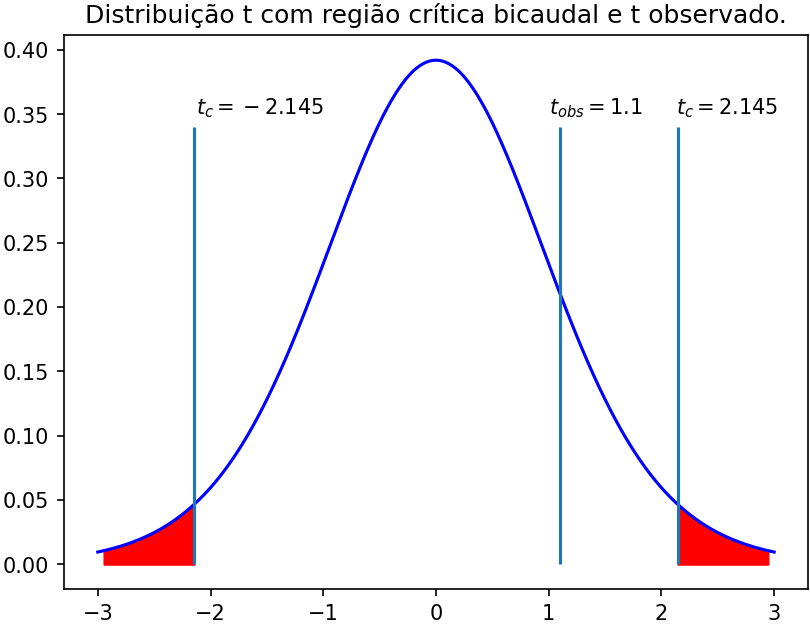
\includegraphics[width=0.55\linewidth]{figs/regiao_critica_bicaudal_t_tobs} \end{center}

\end{frame}


\setbeamercovered{transparent}
\begin{frame}
\frametitle{Etapa 5: calcule o tamanho do efeito e descreva se o seu grau}
Um tamanho de efeito é um índice da diferença entre a média da amostra e a média da população. A estatística de tamanho do efeito normalmente usada ao comparar duas médias é d. 
\begin{align*}
d &= \frac{Desvio\quad observado\quad entre\quad as\quad medias}{Desvio\quad padrao}\\
  &= \frac{\bar{x}-\mu}{DP} = \frac{3160 - 3000}{561.630} = 0.28
\end{align*}

\end{frame}

\setbeamercovered{transparent}
\begin{frame}
\frametitle{Etapa 6: Interpretando os Resultados do Teste de Hipóteses}

Declaração resumida sobre o teste estatístico acima:\\~\\

O salário médio estimado para estudantes típicos de psicologia $(\bar{x} = 3160.00, DP = 561.63)$ não foi significativamente diferente do salário médio mensal real de 3000 Reais, t(14) = 1.10, $p > 0.05$ (bicaudal), d = 0.28. Esses resultados sugerem que os estudantes de farmácia são bastante precisos ao estimar os futuros salários iniciais de outras pessoas.\\~\\

Geralmente, você deve fornecer o valor exato de p, se souber. Em alguns casos, você não saberá disso e então escreveria \("p < 0.05"\) se rejeitou a hipótese nula ou \("p > 0.05"\) se não rejeitou a hipótese nula.
\end{frame}

\setbeamercovered{transparent}
\begin{frame}
\frametitle{Exemplo 8.5}
Deseja-se investigar se uma certa moléstia que ataca o rim altera o consumo de oxigênio desse orgão. Para indivíduos sadios, admite-se que esse consumo tem distribuição Normal com média 12\(cm^3/min\). Os valores medidos em cinco pacientes com a moléstia foram: 14.4, 12.9, 15.0, 13.7 3 13.5. Qual seria a conclusão, ao nível de 1\% de significância?
\vspace{1in}
\vspace{1in}

\end{frame}

\begin{frame}
\frametitle{Distribuição Normal}

\begin{center}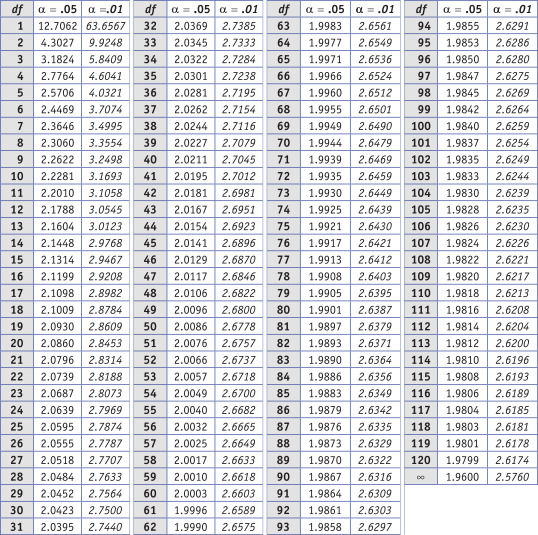
\includegraphics[width=0.7\linewidth]{figs/tabela_t} \end{center}
\end{frame}


\setbeamercovered{transparent}
\begin{frame}
\frametitle{Exemplo 8.3.2}
Uma amostra com 10 observação de uma variável aleatória Normal forneceu média de 5.5 e variância amostral de 4. Deseja-se testar, ao nível de signifiância de 5\%, se a média na população é igual ou menor que 6. Qual a conclusão?
\vspace{1in}
\vspace{1in}

\end{frame}

\setbeamercovered{transparent}
\begin{frame}
\frametitle{Referências bibliográficas}
\printbibliography
\end{frame}

\end{document}